\documentclass[12pt,]{article}
\usepackage[utf8]{inputenc}
\usepackage[T1]{fontenc}
\usepackage{mathptmx}
\usepackage{geometry}
\usepackage{mathtools}
\usepackage{amsmath}
\usepackage[english]{babel}
\usepackage{graphicx}
\usepackage[os=win]{menukeys}
\usepackage[figurename=Gambar]{caption}
\usepackage{hyperref}
\usepackage{minted}
\usepackage{float}
\usepackage{pdflscape}
\usepackage{pdfpages}
\usepackage[yyyymmdd,hhmmss]{datetime}
\usepackage{tikz}

\newcommand{\ShowOsVersion}{%
	\immediate\write18{\unexpanded{foo=`uname -snrmo` && echo "\\verb+${foo}+" > tmp.tex}}%
	\input{tmp}\immediate\write18{rm tmp.tex}%
}

\newcommand{\ShowTexVersion}{%
	\immediate\write18{\unexpanded{foo=`pdflatex -version | head -n1` && echo "\\verb+${foo}+" > tmp.tex}}%
	\input{tmp}\immediate\write18{rm tmp.tex}%
}

\hypersetup{
	colorlinks=true, %set true if you want colored links
	linktoc=all,     %set to all if you want both sections and subsections linked
	linkcolor=blue,  %choose some color if you want links to stand out
}

\geometry{
	a4paper,
	left=15mm,
	right=10mm,
	top=10mm,
	bottom=10mm,
}

\title{\Large \bf
	Laporan Praktikum Uji Audiometri
}

\author{Achmadi ST MT}
\date{}

\begin{document}
	\maketitle
	\thispagestyle{empty}
	\pagestyle{empty}
	
	\vspace*{100px}
	\begin{figure}[H]
		\centering
		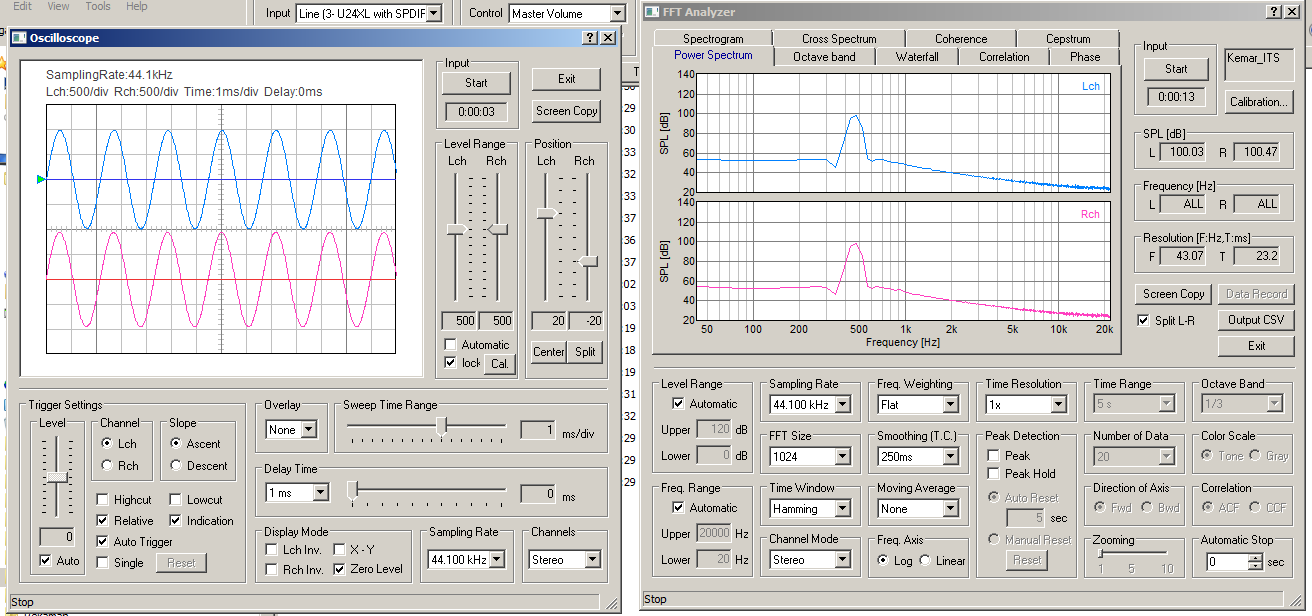
\includegraphics[width=0.9\linewidth]{result/BestResult}
	\end{figure}
	
	\vspace*{200px}
	\noindent This report written using:\\
	OS : \ShowOsVersion \\
	TeX : \ShowTexVersion \\
	Update: {\today} at \currenttime\\
	
	\section{Pendahuluan}
	
	Dokumen ini adalah laporan teknis yang menjabarkan detil pencapaian dari 
	pengembangan unit produk Audiometri yang akan dipasarkan baik kebutuhan medis
	maupun kebutuhan umum. 
	
	\subsection{Requirement}
	
	Berikut akan dijabarkan acuan kebutuhan (\textit{requirement}) yang terbagi dalam 2 kategori, 
	yaitu dari sisi (1) pengguna dan (2) teknis.
	
	\subsubsection{User}
	Requirement dari sisi pengguna adalah rincian kebutuhan dari sudut pandang pengguna.
	Berikut adalah rangkumannya:
	\begin{itemize}
		\item \textbf{Portabel}. Unit produk harus portabel sehingga tidak terikat secara mandatory
		pada suatu posisi/tempat.
		Parameter portabel mengacu antara lain:
		\begin{itemize}
			\item \textbf{Power source}. Unit harus memiliki sumber tenaga sendiri yang tidak terikat posisi/tempat.
			Dapat berupa battery sekali pakai maupun \textit{rechargeable}.
			
			\item \textbf{Ukuran}. Unit harus memiliki ukuran volume kecil dan massa yang ringan.
			Ukuran \textit{hand-held} adalah pilihan tepat.
			
			\item \textbf{Interface}. Unit harus menggunakan \textit{interface} antar muka yang tidak membutuhkan unit
			interface tambahan lain seperti keyboard atau mouse/pointer.
			Dan antar-muka harus terintegrasi dengan unit produk.
			
		\end{itemize}
	
		\item \textbf{Storage}. Unit harus memiliki metode atau part untuk menyimpan hasil pengukuran,
		atau mengirimkan hasil itu ke unit lain yang lebih lazim tersedia
		
		\item \textbf{Intuitif}. Unit harus mengikuti standar produk intuitif sehingga pengguna 
		dapat mengoperasikan unit dengan sedikit atau tanpa sama sekali membutuhkan panduan.
	\end{itemize}
	
	\subsubsection{Teknis}
	
	Berdasarkan kebutuhan pengguna, maka dapat dirangkum kebutuhan dalam \textit{term} lebih teknis.
	Berikut rangkumannya:
	\begin{itemize}
		\item Unit harus menggunakan daya VDD (3.3 volt) atau VCC (5 volt) dengan konsumsi arus rendah.

		\item Unit harus menggunakan komponen seminimal mungkin agar ukurannya kecil dan ringan.

		\item Unit harus dilengkapi \textit{interface} atau antar-muka pengguna.
		Lebih detil:
		\begin{itemize}
			\item Untuk input cukuplah tombol-tombol push button.
			\item Untuk display cukuplah LCD atau LED indikator.
			\item Jika memungkinkan, jadikan satu input dan display
			dalam bentuk layar sentuh LCD-TFT.
		\end{itemize}
		\item Unit harus memiliki emulasi \textit{filesystem} untuk media peyimpanan seperti
		SDCard, MMC, atau USB-Flashdisk.
		
		\item Unit harus menyembunyikan semua kompleksitas teknis sehingga mudah digunakan pengguna.
		Jika membutuhkan perangkat lain maka wajib perangkat tersebut sudah lazim tersedia.
		 
	\end{itemize}
	
	\newpage
	\section{Rancangan}
	
	\subsection{Overview}
	Dengan memperhatikan \textit{requirement} yang telah dijabarkan, maka dapat dibuat rancangan dari pilihan
	komponen-komponen yang telah ada dan tersedia.
	Berikut bagian utama rancangan:
	\begin{itemize}
		\item CPU menggunakan STM32 Cortex-M4.
		Detil pertimbangan:
		\begin{itemize}
			\item ARM 32-bit Cortex-M4. 
			\item Tegangan daya 3.3V.
			\item Ukuran kecil standar paket TQFP.
			\item Tersedia protokol FSMC untuk layar-sentuh LCD-TFT.
			\item Tersedia protokol SPI-FatFs untuk media SDCard/MMC.
			\item Tersedia protokol SPI-I2S untuk Audio PCM.
			\item Tersedia total 144 pin GPIO untuk LED dan tombol.
			\item Harga sangat terjangkau untuk fitur yang tersedia.
		\end{itemize}
		
		\item Audio DAC (Digital to Analog Converter) MAX98357A.
		Detil pertimbangan:
		\begin{itemize}
			\item Class-D Amplifier.
			\item Tegangan daya 3.3V atau 5V tanpa butuh tegangan negatif.
			\item Protokol PCM 16-bit standar I2S (Inter-Integrated Sound).
			\item Output langsung ke coil/speaker tanpa tambahan amplifier lain. 
			\item Tersedia pilihan gain 3dB, 6dB, 9dB (default), 12dB, dan 15dB.
			\item Tersedia fitur Shut-Down untuk \textit{High-Impedance}
			saat tidak menghasilkan output apapun.
		\end{itemize}
	\end{itemize}
	\begin{figure}[H]
		\centering
		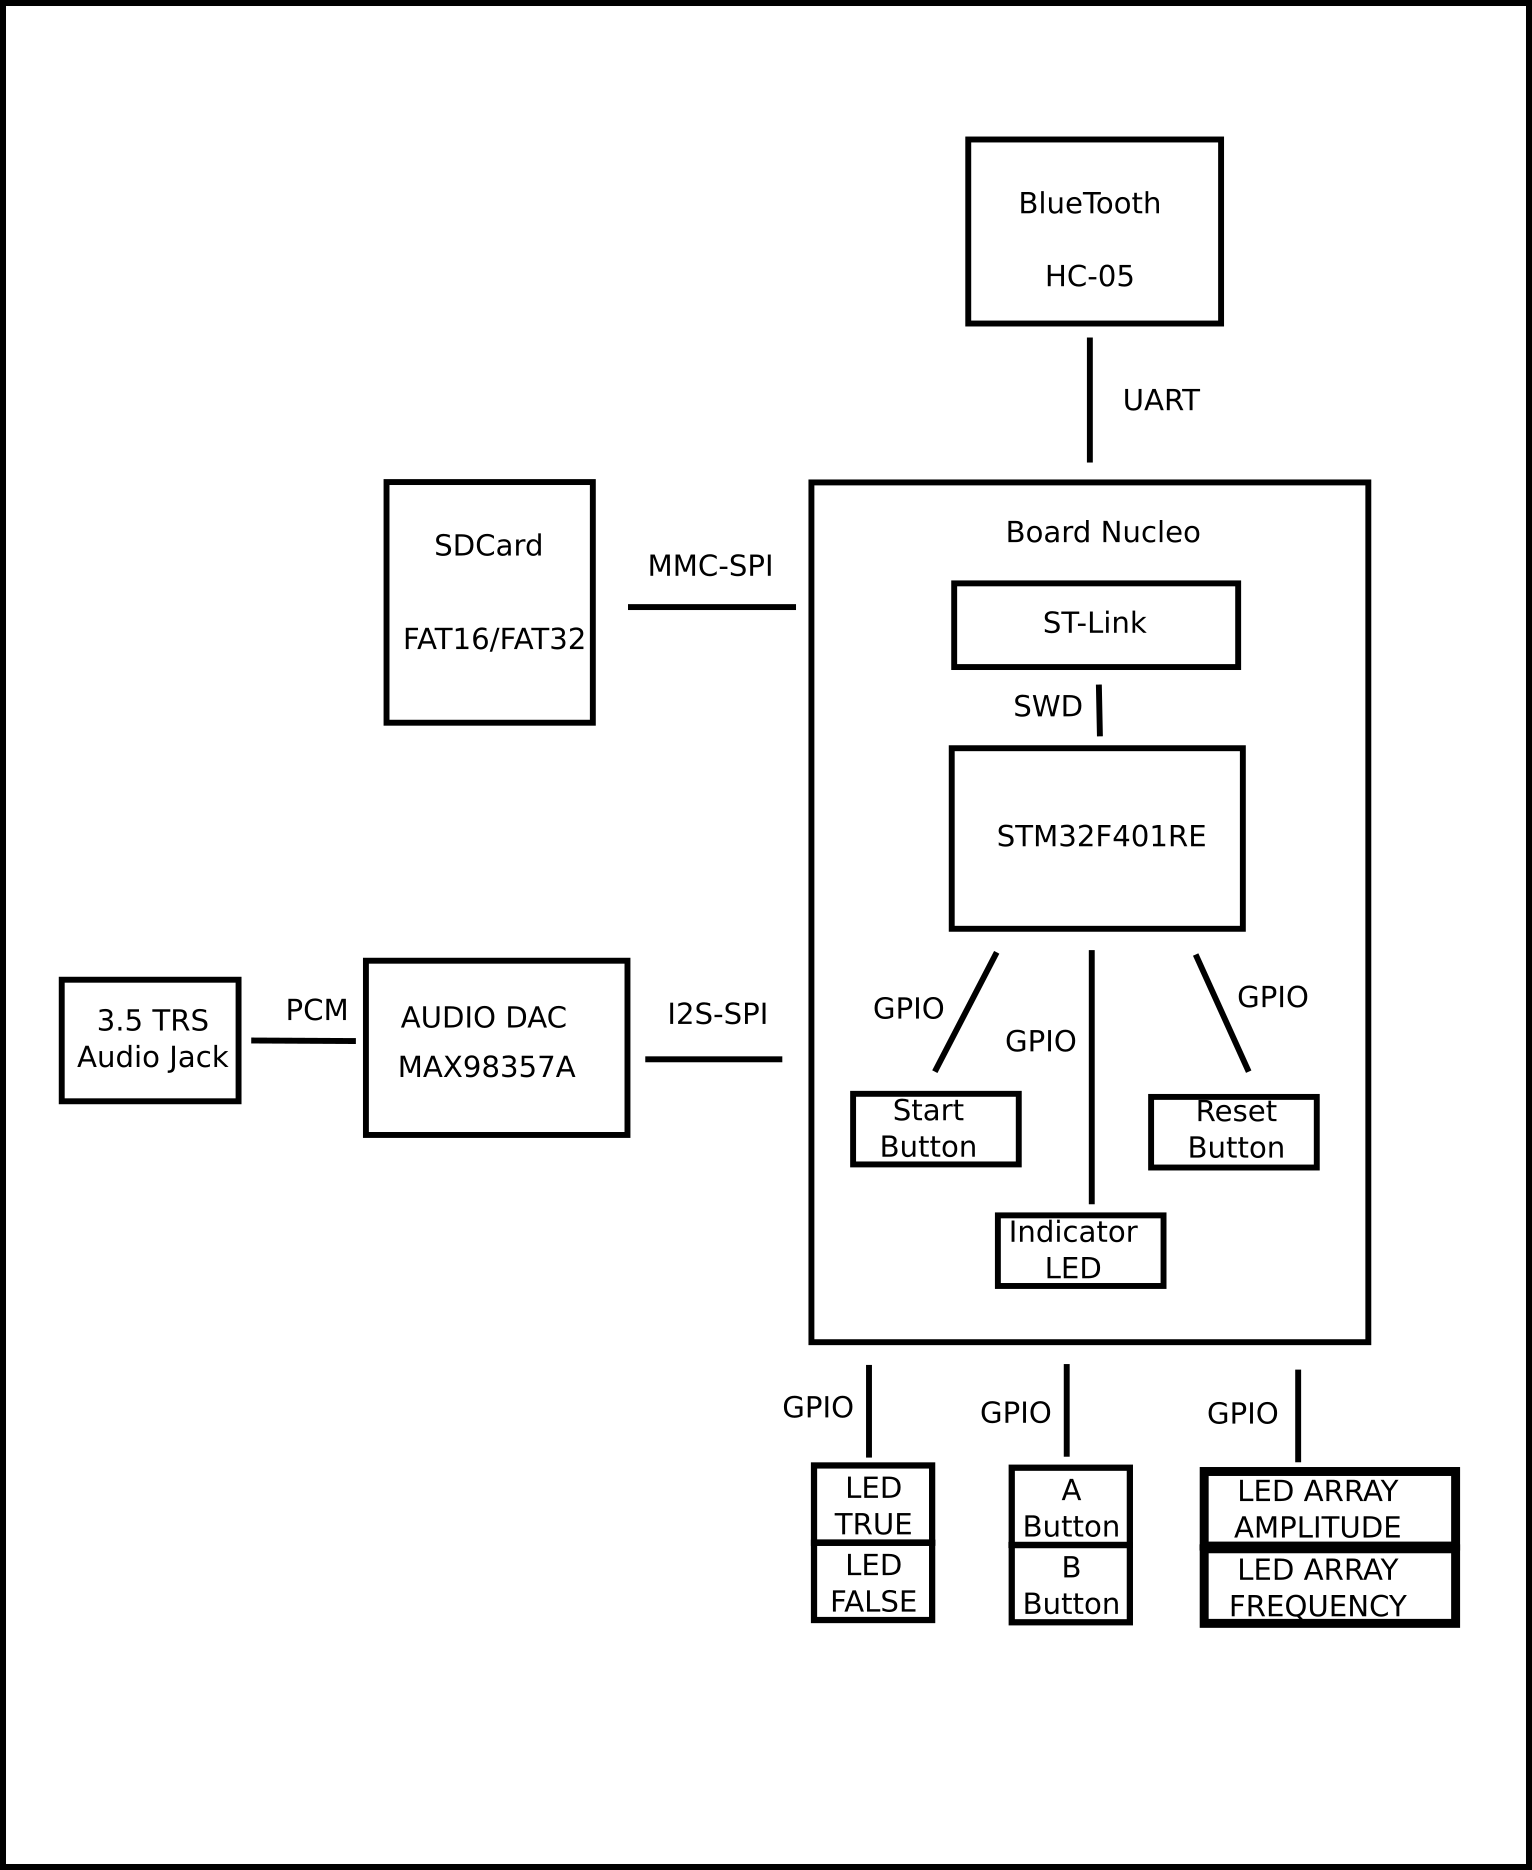
\includegraphics[width=0.6\linewidth]{images/overview}
	\end{figure}

	\newpage
	\subsection{Tone Generator}
	Berikut adalah kelanjutan penjelasan lebih detil tentang bagian tone generator.
	Komponen utama adalah chip STM32 dan Audio DAC MAX98375A.
	
	\subsubsection{PCM 16-bit}
	PCM (\textit{Pulse-Coded Modulation}) adalah protokol standar untuk bertukar data audio digital.
	Setiap satu frame data PCM terdiri dari 32 bit data untuk channel kanan dan kiri masing-masing 16-bit.
	Jumlah frame mengikuti panjang array buffer yang digunakan.
	Berikut diagram sinyal PCM (dokumentasi chip MAX98357A):
	\begin{figure}[H]
		\centering
		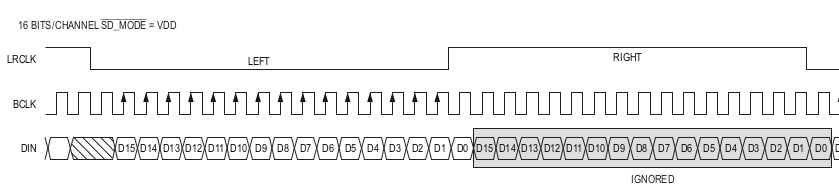
\includegraphics[width=\linewidth]{images/PCM}
	\end{figure}

	Berikut penjelasan 3 sinyal yang dikirim:
	\begin{itemize}
		\item \textbf{LRCLK (Left/Right Clock)}. Sinyal untuk kontrol bagian kanan dan kiri.
		Mengingat chip MAX98357A adalah \textit{mono-amplifier},
		maka posisi sinyal kanan (atau LRCLK berlogika \textit{high}) akan diabaikan.
		
		\item \textbf{BCLK (Bit Clock)}. Sinyal clock untuk kirim data.
		Chip MAX98357A akan membaca nilai bit data di setiap tepi-naik (\textit{Rising-Edge})
		dari sinyal BCLK.
		
		\item \textbf{DIN (Data IN)}. Sinyal bit data. 
		Satu frame 32-bit Left/Right berasal dari satu variabel elemen dari array buffer. 
	\end{itemize}
	
	Di chip STM32, modulasi PCM dikirim melalui protokol I2S (\textit{Inter-Integrated Sound})
	menggunakan jalur komunikasi SPI (\textit{Serial Peripheral Interface}).
	Secara berurutan, koneksi untuk SPI (MOSI-SCK-NSS) dan untuk I2S (DIN-BCLK-LRCLK).
	Untuk chip MAX98357A tidak dibutuhkan sinyal MCLK (Master Clock).
	
	\subsubsection{Class-D Amplifier}
	
	Secara umum, amplifier tipe Class-D adalah jenis amplifier yang tidak mengambil sinyal analog sebagai input.
	Sebaliknya menggunakan sinyal digital PWM (Pulse-Width Modulation) atau PCM (Pulse-Coded Modulation) sebagai input.
	
	Sinyal input ini kemudian ditumpangkan (dimodulasi) ke PWM frekuensi tinggi dan diamplifikasi sesuai nilai gain.
	Kemudian dengan \textit{low-pass filter}, sinyal dikonversi menjadi lebih analog
	dengan membuang PWM frekuensi tinggi yang "tersisa" di output.
	\begin{figure}[H]
		\centering
		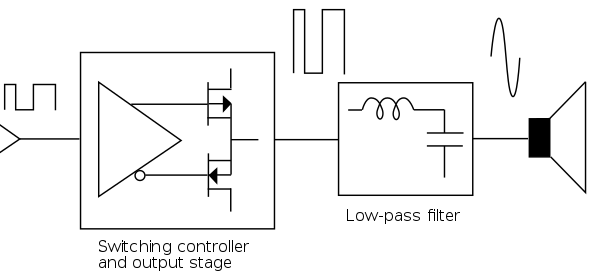
\includegraphics[width=0.6\linewidth]{images/classD}
	\end{figure}

	\newpage
	Chip MAX98357A menggunakan sinyal dasar \textit{squared} PWM pada frekuensi 300kHz.
	Untuk low-pass filter, digunakan Capasitor 220pF dan Ferrit/Inductor.
	\begin{figure}[H]
		\centering
		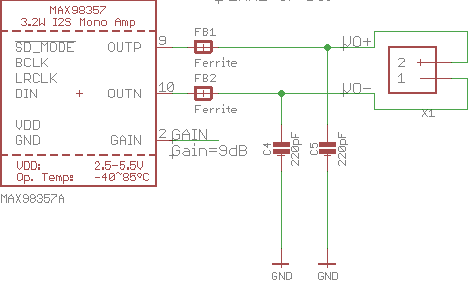
\includegraphics[width=0.6\linewidth]{images/max98357A}
	\end{figure}

	\subsubsection{Programming}
	Berikut adalah penjabaran programming yang digunakan untuk tone generator.
	Penjelasan hanya spesifik untuk protokol I2S tanpa dikaitkan dengan fitur lain.
	Seluruh pustaka/modul programming menggunakan abstraksi dari ChibiOS/RT untuk platform chip STM32F4.
	
	Untuk mempermudah, maka dibagi dalam bagian-bagian utama.
	Berikut rincian:
	\begin{itemize}
		\item Pengaturan clock untuk peripheral SPI-I2S pada default 96 MHz
		\begin{minted}[frame=lines,fontsize=\footnotesize]{c}
#define STM32_PLLM_VALUE    16
#define STM32_PLLN_VALUE    384
#define STM32_PLLP_VALUE    8
#define STM32_I2SSRC        STM32_I2SSRC_PLLI2S
#define STM32_PLLI2SN_VALUE 288
#define STM32_PLLI2SR_VALUE 3
		\end{minted}
		
		\item Variabel array buffer.
		Ukuran variabel adalah 16-bit (sesuai ukuran bit PCM).
		Panjang array total harus cukup panjang untuk menghindari
		noise akibat zero-padding yang tidak tercapai. 
		\begin{minted}[frame=lines,fontsize=\footnotesize]{c}
uint16_t i2s_tx_buf[512*16];
		\end{minted}
		
		\item Variabel Driver I2S.
		Disini dimasukkan variabel array buffer.
		Juga didefinisikan ukuran buffer yang akan di \textit{play-loop}.
		Ukuran buffer play ini harus lebih kecil daripada total array buffer
		dan akan mempengaruhi frekuensi tone yang dihasilkan.
		Ukuran buffer play default adalah 512.
		Frekuensi BCLK diatur pada 16kHz.
		\begin{minted}[frame=lines,fontsize=\footnotesize]{c}
I2SConfig i2scfg = {
	i2s_tx_buf,
	NULL,
	512,
	NULL,
	0,
	16,
};
		\end{minted}
		
		\newpage
		\item Mengatur semua nilai array ke 0.
		Model matematis:
		\[ Y_i = 0, \text{ for } 0 \leq i < 512 \]
		Dan model \textit{array-loop}:
		\begin{minted}[frame=lines,fontsize=\footnotesize]{c}
for(i=0;i<512;i++){
	i2s_tx_buf[i] = 0;
}
		\end{minted}
		
		\item Mengatur sine tone.
		Fungsi ini akan dimodifikasi dan disesuaikan hingga mendapatkan
		tone yang paling bersih pada frekuensi yang lebih tinggi
		dari frekuensi yang diinginkan.
		Model matematis:
		\[ Y_i = sin(2\pi f \frac{i}{512}), \text{ for } 0 \leq i < 512 \]
		Dan model array-loop:
		\begin{minted}[frame=lines,fontsize=\footnotesize]{c}
for(i=0;i<512;i++){
	i2s_tx_buf[i] = sin((double) freq*i*2*(M_PI/512));
}
		\end{minted}
		
		\item \textit{Playing} sine array dalam \textit{looping}
		terus-menerus dalam rentang durasi (dalam detik).
		I2S menggunakan SPI channel 2 sehingga menggunakan driver I2SD2.
		\begin{minted}[frame=lines,fontsize=\footnotesize]{c}
i2sStart(&I2SD2, &i2scfg);
i2sStartExchange(&I2SD2);

chThdSleepMilliseconds(duration*1000);

i2sStopExchange(&I2SD2);
i2sStop(&I2SD2);
		\end{minted}
		
	\end{itemize}

\end{document}